\documentclass{report}

\usepackage{subcaption} % package for subfigures
\usepackage{hyperref}  % package for linking figures etc
\usepackage{enumitem}  % package for description with bullets
\usepackage{graphicx}  % package for importing images
\usepackage{mathtools} % package for math equation
\usepackage{mathrsfs}  % package for math font
\usepackage{indentfirst} % package for getting ident after section or paragraph
\usepackage[export]{adjustbox}
% \usepackage{amsmath}

\setlength{\parindent}{2em} % how much indent to use when we start a paragraph

\graphicspath{ {./theory/figures/} }       % path for images

\begin{document}

\chapter{Classification stage}
\section{Description}
After getting all proposed tubes, it's time to do classification. As classifiers we use 3 approaches
\begin{itemize}
\item  A Recursive Neural Network (RNN) Classifier
\item  A Linear Classifier
\item  A Support Vector Machine (SVM) Classifier
\end{itemize}

The general structure of the whole network is depicted in figure \ref{fig:whole_network}

\begin{figure}[h]
  % 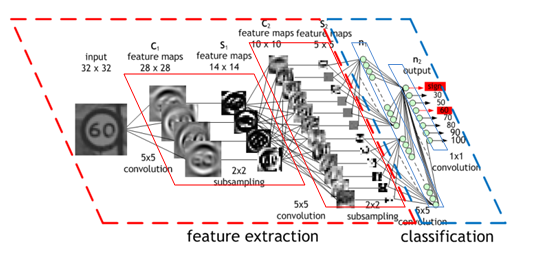
\includegraphics[scale=0.7]{convolutional_neural_network_structure} \]
  \centering
  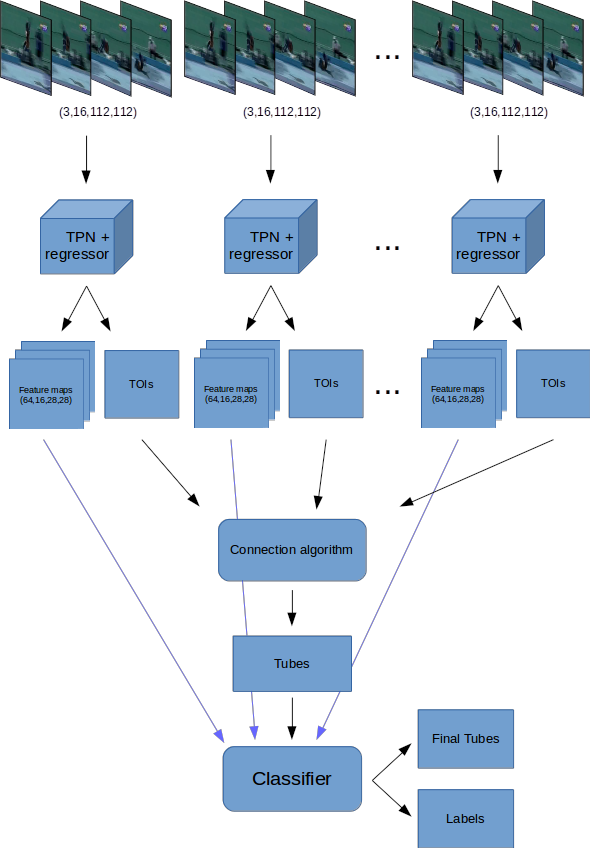
\includegraphics[scale=0.7]{model}
  \caption{Structure of the whole network}
  \label{fig:whole_network}
\end{figure}

\section{ RNN Classifier}
First approach includes a RNN as classifier. The reason is that we do not have a fix temporal size for
each tube. 

\section{Linear Classifier}

Using a Linear classification we follow the next steps:
\begin{enumerate}
\item Firstly we extract the canditate tubes for the whole video and get their corresponding features.
\item For each canditate tube, we get a tensor with dimensions (\#clips,256,\#frames,7,7) where \#frames is
  the number of frames of each clip. So we calculate the average value for all the clips and we get a tensor
  with dimension (256,\#frames,7,7).
\item Our linear Classifier gets as input the previous tensor.
\end{enumerate}

In order to consider a valide classification, we set as confidence threshold equal to 0.5, 0.75 and 0.9 .
We firstly examine our classifier's performance only for jHMDB dataset. 
In figure \ref{} we can see the first results which are disappointed. 

\subsection{Improving results}



\section{Support Vector Machine}
After using Linear Classifier, we used a Support Vector Machine (SVM) in order to classsify our tubes.




\section{Final Improvements}
After classification, we relize that a lot of classified tubes overlap and represent the same action. So, we use again NMS algorithm in order
to remove unnecessary tubes. The new model can be seen in figure \ref{fig:network_nms}.

\begin{figure}[h]
  % 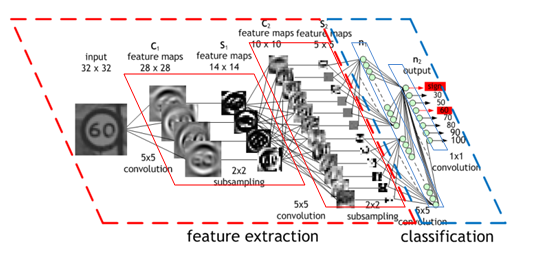
\includegraphics[scale=0.7]{convolutional_neural_network_structure} \]
  \centering
  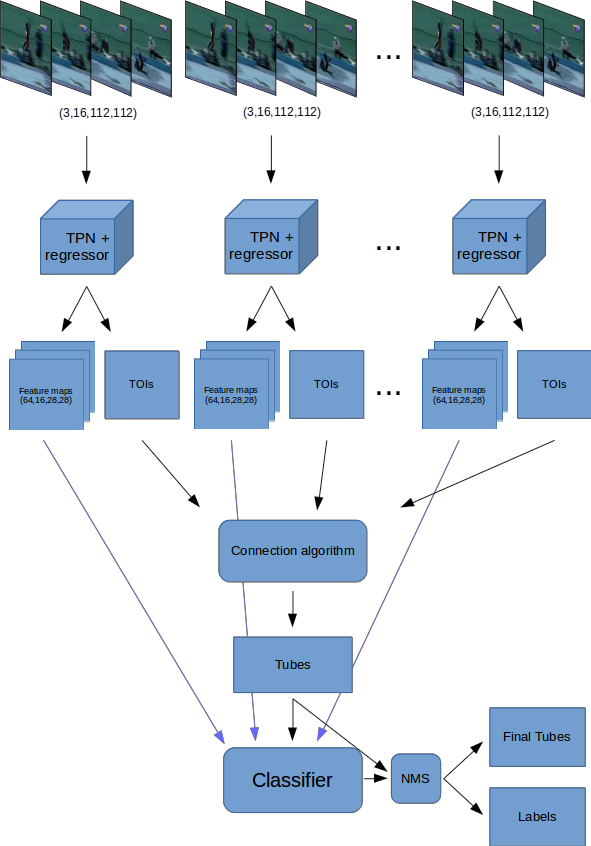
\includegraphics[scale=0.7]{model_nms}
  \caption{Structure of the network with NMS}
  \label{fig:network_nms}
\end{figure}

\end{document}
